
\documentclass[a4paper]{article}
\usepackage[utf8]{inputenc}
\usepackage[T1]{fontenc}
\usepackage{amsmath, amssymb}
\usepackage{xspace}
\usepackage[frenchb]{babel}
\usepackage{hyperref}
\usepackage{graphicx}
\usepackage{caption}
\usepackage{subcaption}
\usepackage{algorithm}
\usepackage{algorithmic}
\usepackage{framed, color}
\definecolor{shadecolor}{RGB}{218,255,202}
\title{Génération de codes d'inférences probabilistes	}
\author{Marvin Lavechin et Pierre Stefani}

\begin{document}
\maketitle
\thispagestyle{empty}

\newpage
\thispagestyle{empty}
\pagenumbering{arabic}
\setcounter{page}{0}
~
\newpage
\tableofcontents

\newpage
 \section{Présentation du projet}
 De Mars à Juillet 2014, encadré par Mr Pierre Henri Wuillemin, chercheur à l'Université Pierre et Marie Curie, nous avons 
 travaillé sur la génération d'un code pour calculer des probabilités d'un réseau bayésien.
 \par \medbreak
 Les réseaux bayésiens sont des faisceaux de probabilités, ordonnés par des liens de parentés. Chacun des événements du réseau bayésien
 possède une table de probabilités dépendant des valeurs prises par ses parents. L'information peut ainsi être diffusé dans de tels réseaux.
 Le projet metaGenBayes utilise cette diffusion, appelé inférence, pour calculer une probabilité spécifique appelé target à partir d'un 
 évènement certain(hard evidence) ou connu(soft evidence). Nous reviendrons sur ce vocabulaire plus en détail par la suite.
 Dans un cadre classique, ce calcul de probabilités selon des observations : $P(X|e)$ est simple. Toutefois, les modèles étant très vite complexes, l'inférence probabiliste devient
 un problème NP-difficile.
 \begin{figure}[h!]
  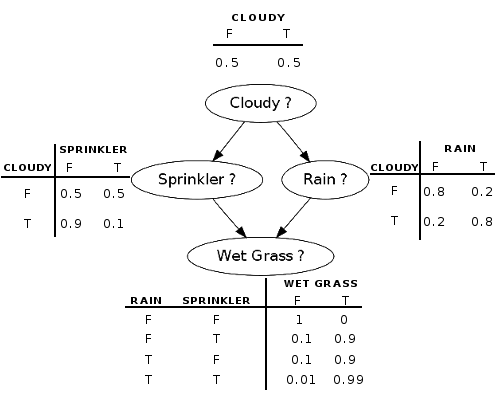
\includegraphics[width=\linewidth]{Images/Waterprinkler.png}
  \caption{Exemple de réseau bayésien}
  \label{fig:bn1}
 \end{figure}
\par \medbreak
Le but du projet était de créer un moteur d'inférence probabiliste, qui n'allait pas faire le calcul mais générer des codes calculatoires dans différents langages cibles. Ce moteur
s'appuie sur certaines bibliothèques lip6, comme par exemple pyAgrum.

\newpage
 \section{Présentation du problème}
  \subsection{Calcul de probabilité}
   \subsubsection{Quelques formules}
   
Comme explicité dans la courte présentation, l'inférence probabiliste s'appuie sur des probabilités conditionnelles, régies par quelques lois de calcul qu'il est important d'introduire:\\
Soient A et B deux événements quelconques d'un même univers. On s'intéresse à ce que devient la probabilité de A lorsqu'on apprend que B est déjà réalisé. On note $P(A|B)$ et on lit "probabilité de A sachant B".
La définition mathématique de $P(A|B)$ est :
$$P(A|B) = \frac{P(A\cap B)}{P(B)} = \frac{P(B|A)P(A)}{P(B)} ,\quad P(B)\ne 0$$
\hfill(Formule de Bayes)
\newline
~
\newline
Cette formule s'écrit aussi :
$P(A|B) \quad \alpha \quad P(A) \times P(B|A)$\footnote{$P(A|B)$ est la loi à posteriori, $P(A)$ la loi à priori et $P(B|A)$ la vraisemblance, tandis que P(B) sert de coefficient normalisateur}
\newline
Ceci nous amène à considérer deux autres formules.
Soit $(A_i)_{i\in I}$ un système complet d'événements de probabilités non nulles. Alors pour tout événement $B$ on a : 
$$P(B)=\sum_{i\in I} P(A_i\cap B)=\sum_{i\in I} P(A_i)P(B|A_i)$$
\hfill(Formule des probabilités totales)
\newline
~
\newline
Si $P(A_1 \cap \ldots \cap A_n) \ne 0$, on a :
$$P(A_1 \cap \ldots \cap A_n) = \prod_{i = 1}^{n} P(A_i|A_{i+1} \cap \ldots \cap A_n)$$
\hfill(Formule des probabilités composées)

    \subsubsection{Calcul au sein d'une table de probabilité jointe}
Soient $A_1,A_2,A_3$ trois variables aléatoires binaires. On peut écrire une table listant toutes les combinaisons possibles de ces 3 variables, qui sont au nombre de $2^3$.\newline
En effet, on a :
\begin{align*}
\begin{pmatrix} A_1 = true & A_2 = true & A_3 = true\end{pmatrix}\\
\begin{pmatrix} A_1 = false & A_2 = true & A_ 3 = true\end{pmatrix} \\
\begin{pmatrix} A_1 = true & A_2 = false & A_ 3 = true\end{pmatrix} \\ etc...
\end{align*}
Pour chacune des combinaisons, supposons que nous disposions de la probabilité jointe de cette combinaison.\newline
Si l'on veut la probabilité $P(A_1 \cap A_2)$, la formule des probabilités totales nous dit qu'il suffit qu'on somme les probabilités des combinaisons de la table pour laquelle $A_1$ est vrai et $A_2$ l'est aussi.
\newline
Si l'on veut la probabilité $P(A_1|A_2)$, la formule de Bayes nous dit qu'il suffit qu'on somme toutes les probabilités des combinaisons de la table pour lesquelles $A_1$ est vrai et $A_2$ est vrai en divisant
par la somme des probabilités des combinaisons de la table pour lesquelles $A_2$
est vrai.
\newline
On peut donc à partir de la table des probabilités jointes déduire n'importe quelle probabilité conditionnelle. Les tailles de ces tables évoluant de manière exponentielle, il devient impossible d'utiliser
simplement cette approche pour le calcul d'inférences probabilistes.

 \subsection{Arbres de Jonction}
Avant de revenir en détail sur les méthodes utilisés pour calculer ces probabilités conditionnelles, nous allons décrire le principe des arbres de jonctions, transformation nécessaire des réseaux bayésiens
en arbres dépourvus de toute orientation. La motivation principale de cette étape est de créer des cliques - noeuds regroupants plusieurs probabilités/évènements de notre réseau. Ces cliques seront alors
liées sans aucune orientation (évitant ainsi la gestion des cycles). Ces arbres doivent également satisfaire la propriété suivante des arbres de jonctions: \\
\textit{Deux cliques U et V possédant un ensemble S de probabilités communes, sont séparés, lors de leur liaison dans l'arbre de jonction, par cet ensemble S}
\begin{figure}[h!]
 \centering
 \begin{subfigure}{.5\textwidth}
  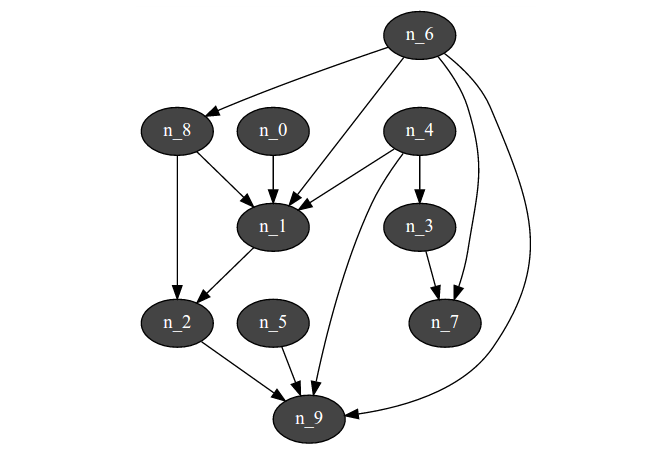
\includegraphics[width=\linewidth]{Images/Bayesian_Network.png}
  \label{fig:bng}  
 \end{subfigure}%
\begin{subfigure}{.5\textwidth}
  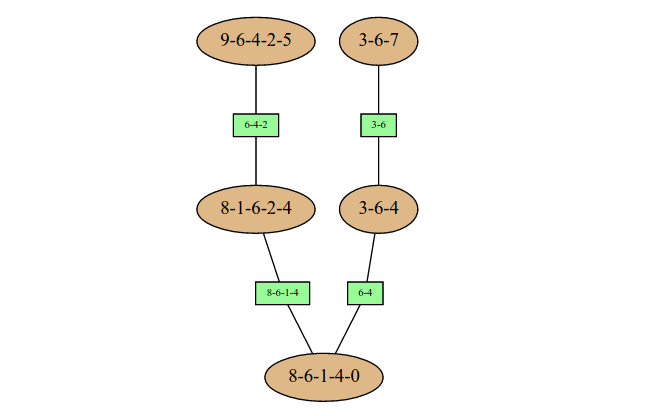
\includegraphics[width=\linewidth]{Images/Junction_Tree.png}
  \label{fig:jtg}  
 \end{subfigure}
 \caption{Un réseau bayésien généré (à gauche), et un arbre de jonction possible pour ce réseau (à droite)}
\end{figure}
\par \medbreak 
La première étape de création de ces arbres est une phase de \textit{moralisation} : il s'agit de créer un lien entre deux parents d'un même élémént. Dans l'exemple de la Figure 2, un lien est crée entre n2 et n5, 
deux des parents de n9. Une fois cette moralisation effectuée, la création de \textit{supercliques} regroupant des élèments connectés du réseau bayésien est quasiment finie. Toute orientation est ensuite enlevée, et la dernière
étape est une phase dite de 'triangulation', pour enlever toute possibilité de cycles à la nouvelle structure. Les arbres de jonctions regroupent désormais plusieurs probabilités, et l'on associera à ces ensembles 
leurs probabilités respectives avec des \textit{potentiels} dans le lexique des réseaux bayésiens, qui seront simplement des tableaux de probabilités dans nos langages plus courants.

  \subsection{Diffusion des probabilités dans les arbres de jonctions}
Rappelons notre principal objectif: à partir d'une évidence donnée pour une probabilité A, nous devons calculer la nouvelle probabilité de l'évènement B: l'information de A va donc devoir circuler dans le réseau. La 
structure d'arbres de jonctions va grandement simplifier ce que l'on appelera la \textit{diffusion} de l'information. La clique de départ, celle pour laquelle  a été transmise l'information
(ce choix arbitraire n'a d'influence que sur le temps de réponse du programme) possède un potentiel $\Phi$ contenant les probabilités des variables de notre réseau. Pour passer d'une clique A à la clique B, 
l'information est projetée de A à B selon les séparateurs comme le montre la Figure 3. 
 \begin{figure}[h!]
  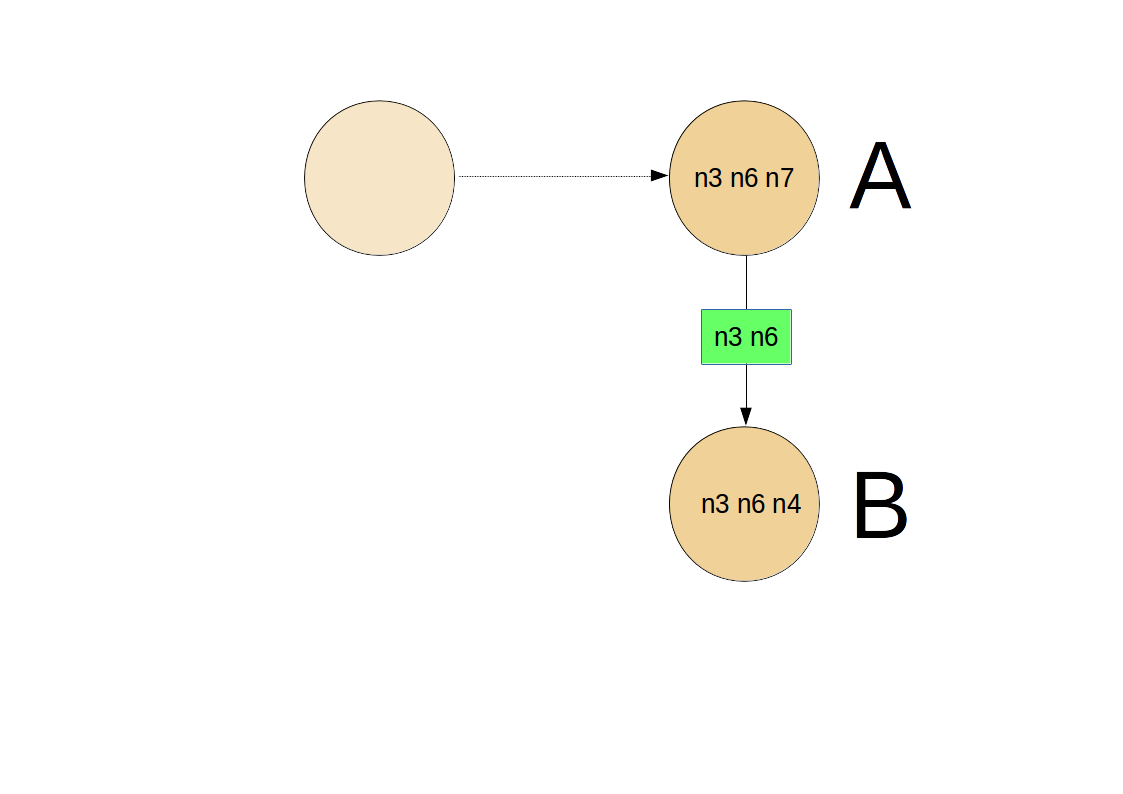
\includegraphics[width=\linewidth]{Images/Diff_Jt.png}
  \caption{Exemple de diffusion d'une clique A vers une clique B dans un arbre de jonction}
  \label{fig:Diff_Jt}
 \end{figure}
\par \medbreak
La projection de A sur B suit d'abors la formule de projection sur le séparateur :\\ $$\Psi_{AB}^{'} = \sum\nolimits_{X_i \in \Phi_{A}, X_i \notin \Psi_{AB}} \Phi_{A}$$  Puis du séparateur à la clique B :\\
$$\Phi_{B}^{'} = \Phi_{B} * \Psi_{AB}^{'}$$ Dans le cas de la figure 3, cela donne: \\
$$\Phi_{n3,n6,n4}^{'} = \Phi_{n3, n6, n4} * \sum\nolimits_{n7} \Phi_{n3, n6, n7}$$\\
Ainsi, à partir des évidences fournies à certaines cliques de l'arbre de jonction, toute l'information sera diffusée vers une clique principale, appelée clique racine, dans une étape que nous avons appelée 
\textit{l'absorption}. Voici l'algorithme utilisé pour définir cette clique racine, vers qui tout converge :
\begin{algorithm}
 \caption{Trouver la clique racine}
 \begin{algorithmic}
  \STATE $VoisinsMax = -1$
  \FOR{$I \in cliques$}
    \FOR{$X \in targets$}
      \IF {$X \in variables(I)$}
	\IF{$nbVoisins(I) > voisinsMax$}
	  \STATE $VoisinsMax \leftarrow nbVoisins(I)$
	  \STATE $CliqueRacine \leftarrow I$
	\ENDIF
      \ENDIF
    \ENDFOR
  \ENDFOR
  \RETURN CliqueRacine
 \end{algorithmic}
\end{algorithm}
\\
Cet algorithme permet à la fois à la clique racine de contenir au moins une target, et donc permettra un calcul rapide pour au moins un résultat, et également d'avoir le maximum de voisins, nous assurant 
ainsi qu'il ne s'agira pas d'une clique isolée pour laquelle de nombreux calculs inutiles seraient effectués. 
\par \medbreak
Il faut pour calculer la probabilité de la target, revenir sur une clique la contenant, et appliquer une marginalisation:\\
Soit une target $T \in C$, une clique de notre arbre. Marginaliser revient à calculer :
$$P(T) = \sum\nolimits_{X \in C, X\neq T} \Phi_{C}$$ \\
Une fois la phase d'absorption effectuée, notre arbre est dans l'état suivant: toute l'information a convergée et est contenue dans une clique racine. C'est à partir de celle-ci que la seconde étape commence,
la \textit{diffusion} vers les targets, pour y appliquer les marginalisations. Une fonction du module \textbf{Compiler} -que nous développerons plus tard, crée une liste de diffusion avec les cliques
visitées contenant les targets. 

\begin{figure}[h!]
 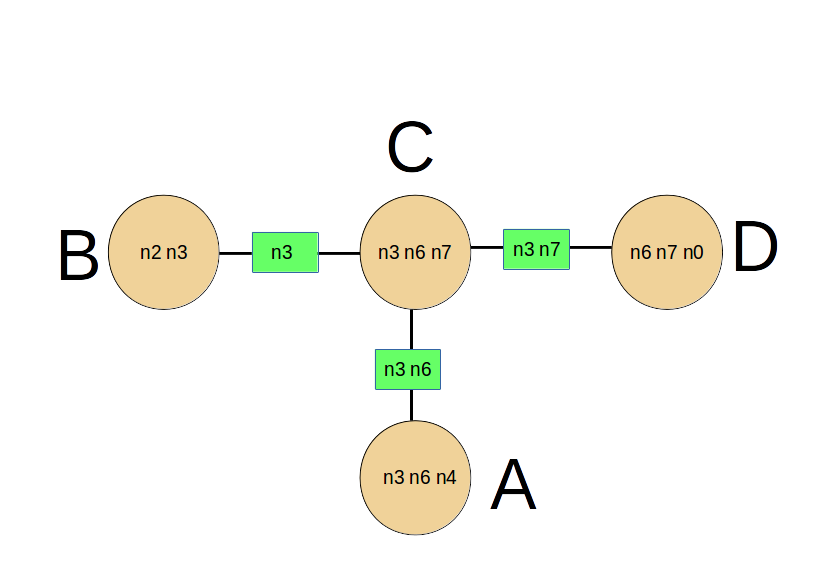
\includegraphics[width=\linewidth]{Images/Diff_Jt2.png}
 \caption{Exemple pour la phase de collecte d'informations de la diffusion}
 \label{fig:Diff_Jt2}
\end{figure}

Admettons que B et C aient reçu l'information de la diffusion, qui doit maintenant être projetée sur A, clique contenant une target. Il faut 'collecter' l'information dans les cliques voisines, c'est à dire, pour
aller de C à A, récupérer les potentiels $\Phi_{B}$ et $\Phi_{D}$, en plus de $\Phi_{C}$. Une fois $\Phi_{C}$ actualisé de la sorte, on peut appliquer les formules de projections sur le séparateur puis vers D 
comme vu précedemment. La clique D et ses potentiels ont alors bien reçu l'information de tout le réseau bayésien.

\section{Description générale du projet}
 \subsection{Présentation de la structure du projet}
 
Ce projet de génération de code calculatoire a été écrit en python, s'appuyant notamment sur la bibliothèque pyAgrum du département lip6. Parmi les langages implémentés pour la génération, on trouve deux versions
Python : une utilisant des fonctions pré-conçues dans pyAgrum, l'autre, plus générale, utilise des tableaux numpy; PHP et Javascript complètent la liste de ces langages. Ce projet nous a donc permis non seulement
d'apprendre comment mener ce genre de travaux: écriture, commentaire, gestion du temps et du travail, mais aussi de nous familiariser avec ces nouveaux langages: une étude plus approfondie de Python était 
nécessaire, et il était important de connaître et comprendre les bases de PHP et Javascript. \\
L'éxècutable final est un fichier Python, \textit{metaGenBayes.py}, qui récupère les spécifités et les requêtes dans un fichier Yaml, support conçu pour ce genre d'utilisation. Ce dernier se présente ainsi:
\begin{itemize}
 \item Un réseau bayésien a donner en entrée, le chemin est relatif au fichier \textit{config.py} fourni avec \textit{config.yaml}.
 \item Les évidences : hard et soft evidences sont supportées par le programme, mais doivent être donnés sous forme de dictionnaires python, suivi, pour les soft evidences, du tableau de valeurs prises par celles-ci,
et pour les hard evidences, de l'indice pour lequel la valeur est certaine. 
 \item Les targets
 \item Le langage ('debug' est un langage supporté, il liste les actions effectuées par le programme)
 \item Le nom de lu fichier généré, qui contiendra les instructions.
 \item Le nom de la fonction principale du fichier créé.
 \item Eventuellement, un header pour le fichier généré.
\end{itemize}
Ce fichier permet de donner au système tous les inputs nécessaires à la construction des fonctions, des fichiers, etc par le compilateur et le générateur du projet. Plus aucune entrée ne sera demandée,
et le fichier obtenu en sortie sera configuré comme souhaité par l'utilisateur.\\

  \subsection{La Compilation}

Pour pouvoir générer en différents langages une même requête, il était nécessaire de passer par une étape dite de compilation, entre les entrées de l'utilisateur et l'écriture dans le langage
spécifié. Le résultat de la compilation, un tableau d'instructions, est compréhensible par tous les langages, et le déchiffrage de ce dernier correspondra à la \textit{génération}. A partir de nos connaissances
en réseaux bayésiens, et après avoir travaillé sur quels types de calculs nous allions devoir utiliser, sept opérations de bases sont apparues. Ce sont ces opérations que l'on retrouve dans chacun des index
du tableau d'instructions, avec leurs arguments. Voici un example d'instruction pour la création d'un potentiel $\Phi_{0 1 3 5}$ contenant les variables 0, 1, 3 et 5 du réseau bayésien:
\begin{snugshade} [ 'CPO', $'Phi-0-1-3-5'$, [0,1,3,5] ]  \end{snugshade}. Voici les opérations principales:
\begin{itemize}
 \item L'initialisation des cpts (probabilités de chacune des variables). Instruction particulière avant toute générétion, permettant la copie dans des variables locales des tableaux de probabilités 
 du réseau bayésien.
 \item La création d'un potentiel, code CPO, qui crée un potentiel dont le \textit{nom} et les \textit{variables} qu'il contient sont passés en paramètres.
 \item L'instruction ASE, qui initialise un potentiel lié à une évidence. Le \textit{nom}, la \textit{valeur} et enfin l'\textit{index} de l'évidence dans le dictionnaire sont les arguments.
 \item La multiplication d'un potentiel par une cpt, MUC. Pour la génération, le \textit{nom} du potentiel, ses \textit{variables} sont stockés, ainsi que la \textit{variable} dont le tableau de probabilités
 sera récupéré.
 \item La multiplication entre deux potentiels, MUL. Là encore, \textit{noms} et \textit{variables} sont ajoutés au tableau d'instruction.
 \item L'instruction MAR pour la marginalisation d'un potentiel selon un autre potentiel. Les mêmes paramètres que pour la multiplication entre deux potentiels sont stockés.
 \item La normalisation d'un potentiel, identifié par son \textit{nom}.
\end{itemize}
Le fichier compiler.py comprend un métacode qui effectue les opérations nécessaires pour ajouter correctement les instructions au tableau petit à petit. 
    \subsubsection{Opérations préalables}
Avant de commencer à définir les potentiels à créer, les chemins de diffusion, etc, deux opérations sont nécessaires au bon fonctionnement du métacode.\\
\textbf{D'une hard evidence à une soft evidence}\\
Dans le langage probabiliste, on distingue deux types d'informations sur une proobabilité. Une soft evidence est une vraisemblance dont on connait chacune des valeurs. Par exemple, si la probabilité
qu'il pleuve aujourd'hui selon qu'il fasse beau, couvert ou orageux est : $P(Pluie|Temps) = [ 0.1, 0.5, 0.8 ]$. Celles-ci sont directement implémentables, en passant le tableau de 
valeurs au potentiel de l'évidence. L'autre type de vraisemblance, l'hard evidence, est une certitude. Avant toute opération de compilation, on transforme l'input hard evidence en un tableau de valeurs
plus classiques où toutes les probabilités sont nulles sauf la certitude, qui vaut 1.
\\
\textbf{Choix d'une clique principale}
Comme vu dans la présentation, le coeur de la compilation repose dans l'absorption de l'information par une clique qui diffusera ensuite vers les cliques contenant les targets. Le choix de cette
clique racine est important pour le temps de calcul du programme. Une première séléction se fait sur les cliques contenant une target, évitant ainsi au moins un parcours de diffusion dans l'arbre de 
jonction. Parmi les cliques candidates, celle ayant le maximum de voisins est choisie, optimisant la diffusion de l'information.\\
  \subsubsection{Création et Initialisation des potentiels}
Dans la bibliothèque pyAGrum, conçue pour travailler avec réseaux bayésiens et arbres de jonctions, chaque clique est considéré comme un potentiel, initialisé avec la commande \textit{pyAgrum.potential()}
sur lequel peuvent s'appliquer les fonctions préconçues de multiplication, marginalisation etc de la bibliothèque pyAgrum. Ces structures n'existant pas dans les autres langages, il faudra initialiser
les potentiels de cliques sous forme de tableaux de probabilités. C'est le but de la première partie du métacode de compilation, qui va parcourir l'arbre de jonction, sachant les évidences fournies et 
les targets demandés, et donnera au tableau d'instructions les variables à créer. Lors de la diffusion de l'information, comme vu dans l'exemple de la figure 4 un peu plus haut, il est nécessaire de collecter
l'information, et donc les potentiels, des cliques environnantes afin de diffuser vers la clique suivante. Or, ces potentiels environnants seront modifiés lors du calcul, puisqu'ils diffusent eux aussi de l'information.
Afin de garder une version inaltérée du tableau de probabilités d'une clique, nous créeons en plus des potentiels dits de diffusion, c'est ceux-ci qui seront modifiés.
  \subsubsection{Absorption et Diffusion de l'information}
Le métacode commence par appeler la fonction \textit{parcours} qui va parcourir en profondeur l'arbre de jonction et créer deux listes: une pour l'absorption, l'autre pour la diffusion. Cette fonction récurrente
commence depuis la clique racine et retourne un booléen. Elle séléctionne d'abord ses voisins, et vérifie si ceux-ci contiennent une target pas encore rencontrée (une liste des targets est progressivement
mise à jour). Si c'est le cas, un couple (clique, target) est enregistré pour signifier à la diffusion que cette clique contient ou mène vers une target. L'appel récursif permet donc d'obtenir une liste 
d'absorption qui signalera au métacode le chemin à suivre jusqu'à la clique racine, puis une liste de diffusion qui elle donne le chemin de la clique racine vers les cliques les plus proches contenant les targets.
\\Ci-dessous un exemple, avec un arbre de jonction où les cliques jaunes contiennent une information/évidence, la clique rouge fait partie des cliques targets, avec la clique numéro 1, clique racine et donc contenant une target également.
\begin{figure}[h!]
 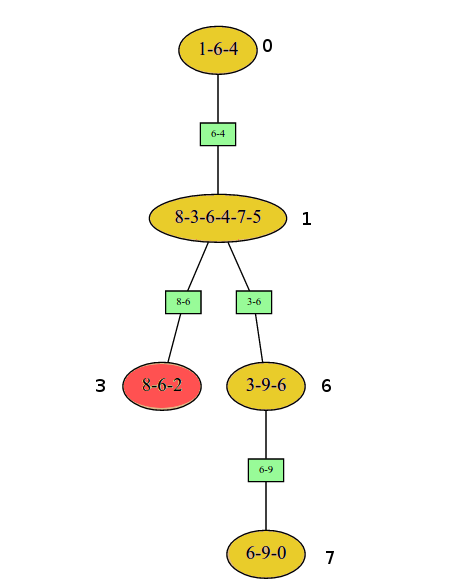
\includegraphics[width=\linewidth]{Images/Parcours.png}
 \caption{Arbre de jonction. Les cliques en jaunes contiennent une évidence, la clique rouge et la clique 1 contiennent des targets.}
 \label{fig:Parcours}
\end{figure}
\\Voici les listes d'absorption et diffusion renvoyés par l'algorithme parcours : 
\begin{snugshade} Absorption : [[0, 1], [3, 1], [7, 6], [6, 1]]; Diffusion : [[1, 3]]  \end{snugshade}
Une fois ces listes correctement définies, elles entrent en paramètres des fonctions suivantes du métacode, qui détermineront les opérations à effectuer pour l'inférence, c'est à dire la transmission de l'
information selon le chemin voulu. Un premier parcours de la liste d'absorption crée les potentiels de séparateurs pour l'envoi d'un message d'une clique à une autre. Comme vu dans la partie
théorique plus haut, pour cette opération, nous devons marginaliser le potentiel séparateur selon la clique 'émettrice' puis multiplier le potentiel de la clique 'réceptrice' par ce potentiel séparateur
marginalisé. La fonction \textit{sendMessAbsorb} réalise toute ces opérations. Aprés l'ajout de la commande de création du potentiel séparateur au tableau d'instruction, la fonction détermine l'intersection 
des deux cliques concernées pour créer le potentiel du séparateur, avant d'ajouter les consignes de marginalisation et multiplication selon les bon potentiels de cliques. Les potentiels sont correctement 
récupérés par l'identifiant unique du tableau d'absorption. Illustrons à nouveau avec un exemple clair: \\
\begin{figure}[h!]
 \centering
 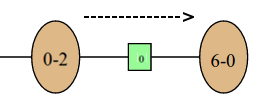
\includegraphics[width=0.5\textwidth]{Images/SendMessAbsorp.png}
 \caption{Deux cliques et leurs variables, et un message à passer par le séparateur.}
 \label{fig:sendMessAbsorb}
\end{figure}
A ce stade de la compilation, le métacode parcourt la liste pour l'absorption et arrive à cet étape, où l'information doit être transmise du potentiel $\Phi_{0-2}$ au potentiel $\Phi_{6-0}$. Une consigne
pour la création du potentiel séparateur est crée, $\Psi_{0-2>6-0}$, et les variables du séparateur y sont ajoutés: la variable 0 ici. Ensuite, on ajoute au tableau d'instructions les commandes de marginalisation selon
la clique 2-0 : [MAR, $\Psi_{0-2>6-0}$, $\Phi_{0-2}$, [0], [2,0]] et de multiplication de la clique 6-0 par le séparateur: [MUL, $\Phi_{6-0}$, $\Psi_{0-2>6-0}$, [6,0], [0]]. \\
Ainsi, toute l'information sera absorbée par la clique racine selon le chemin défini. \\
Passons à la diffusion vers les targets. Si diffusion il y a (elle n'a pas lieu d'être si une seule target est demandé par exemple), un algorithme similaire à celui de l'absorption régit le passage de l'information
d'une clique à l'autre. Les instructions de création de potentiel séparateur sont ajoutées, les variables du séparateur y sont insérées. Comme vu précedemment, l'information doit être collecté dans les cliques
voisines avant de pouvoir passer à la clique suivante. Une fonction de collecte a donc été implémenté, qui récupère l'information de tous les voisins d'une clique donnée, sauf un, passé en argument, et qui est
dans notre cas la clique vers qui l'inférence est effectuée.
Une première étape consiste à définir les potentiels - et donc futurs variables- à créer et comment les initialiser.
Toutes ces instructions donnent un tableau utilisable par les modules de génération qui ont été implémentés par la suite. Leurs arguments permettent de récupérer des informations capitales lors de l'écriture
des codes calculatoires et d'effectuer quelques opérations dans la phase suivante. Toutefois, à cet instant là de l'éxécution, la grande majorité des opérations ont été faites. \\

\end{document}